% Preamble
\documentclass{beamer}
\usepackage[utf8]{inputenc}
\usepackage{german}
\usepackage{ngerman}

\title[TSP]
{Travelling Salesman Problem}
\subtitle{Exakte Lösungen}
\author
{Axel Christ}
\institute{DHBW Karlsruhe}
\subject{Theorieseminar Informatik}

\AtBeginSection[]
{
  \begin{frame}
    \frametitle{Table of Contents}
    \tableofcontents[currentsection]
  \end{frame}
}

\begin{document}
  \frame{\titlepage}
  \section{Definition}
  \begin{frame}
    \frametitle{Definition}
    Ein Handlungsreisender muss mehrere Städte besuchen. Dabei soll die
    Strecke, um alle Städte zu besuchen, möglichst kurz sein.
    \pause
    \begin{figure}
      \centering
      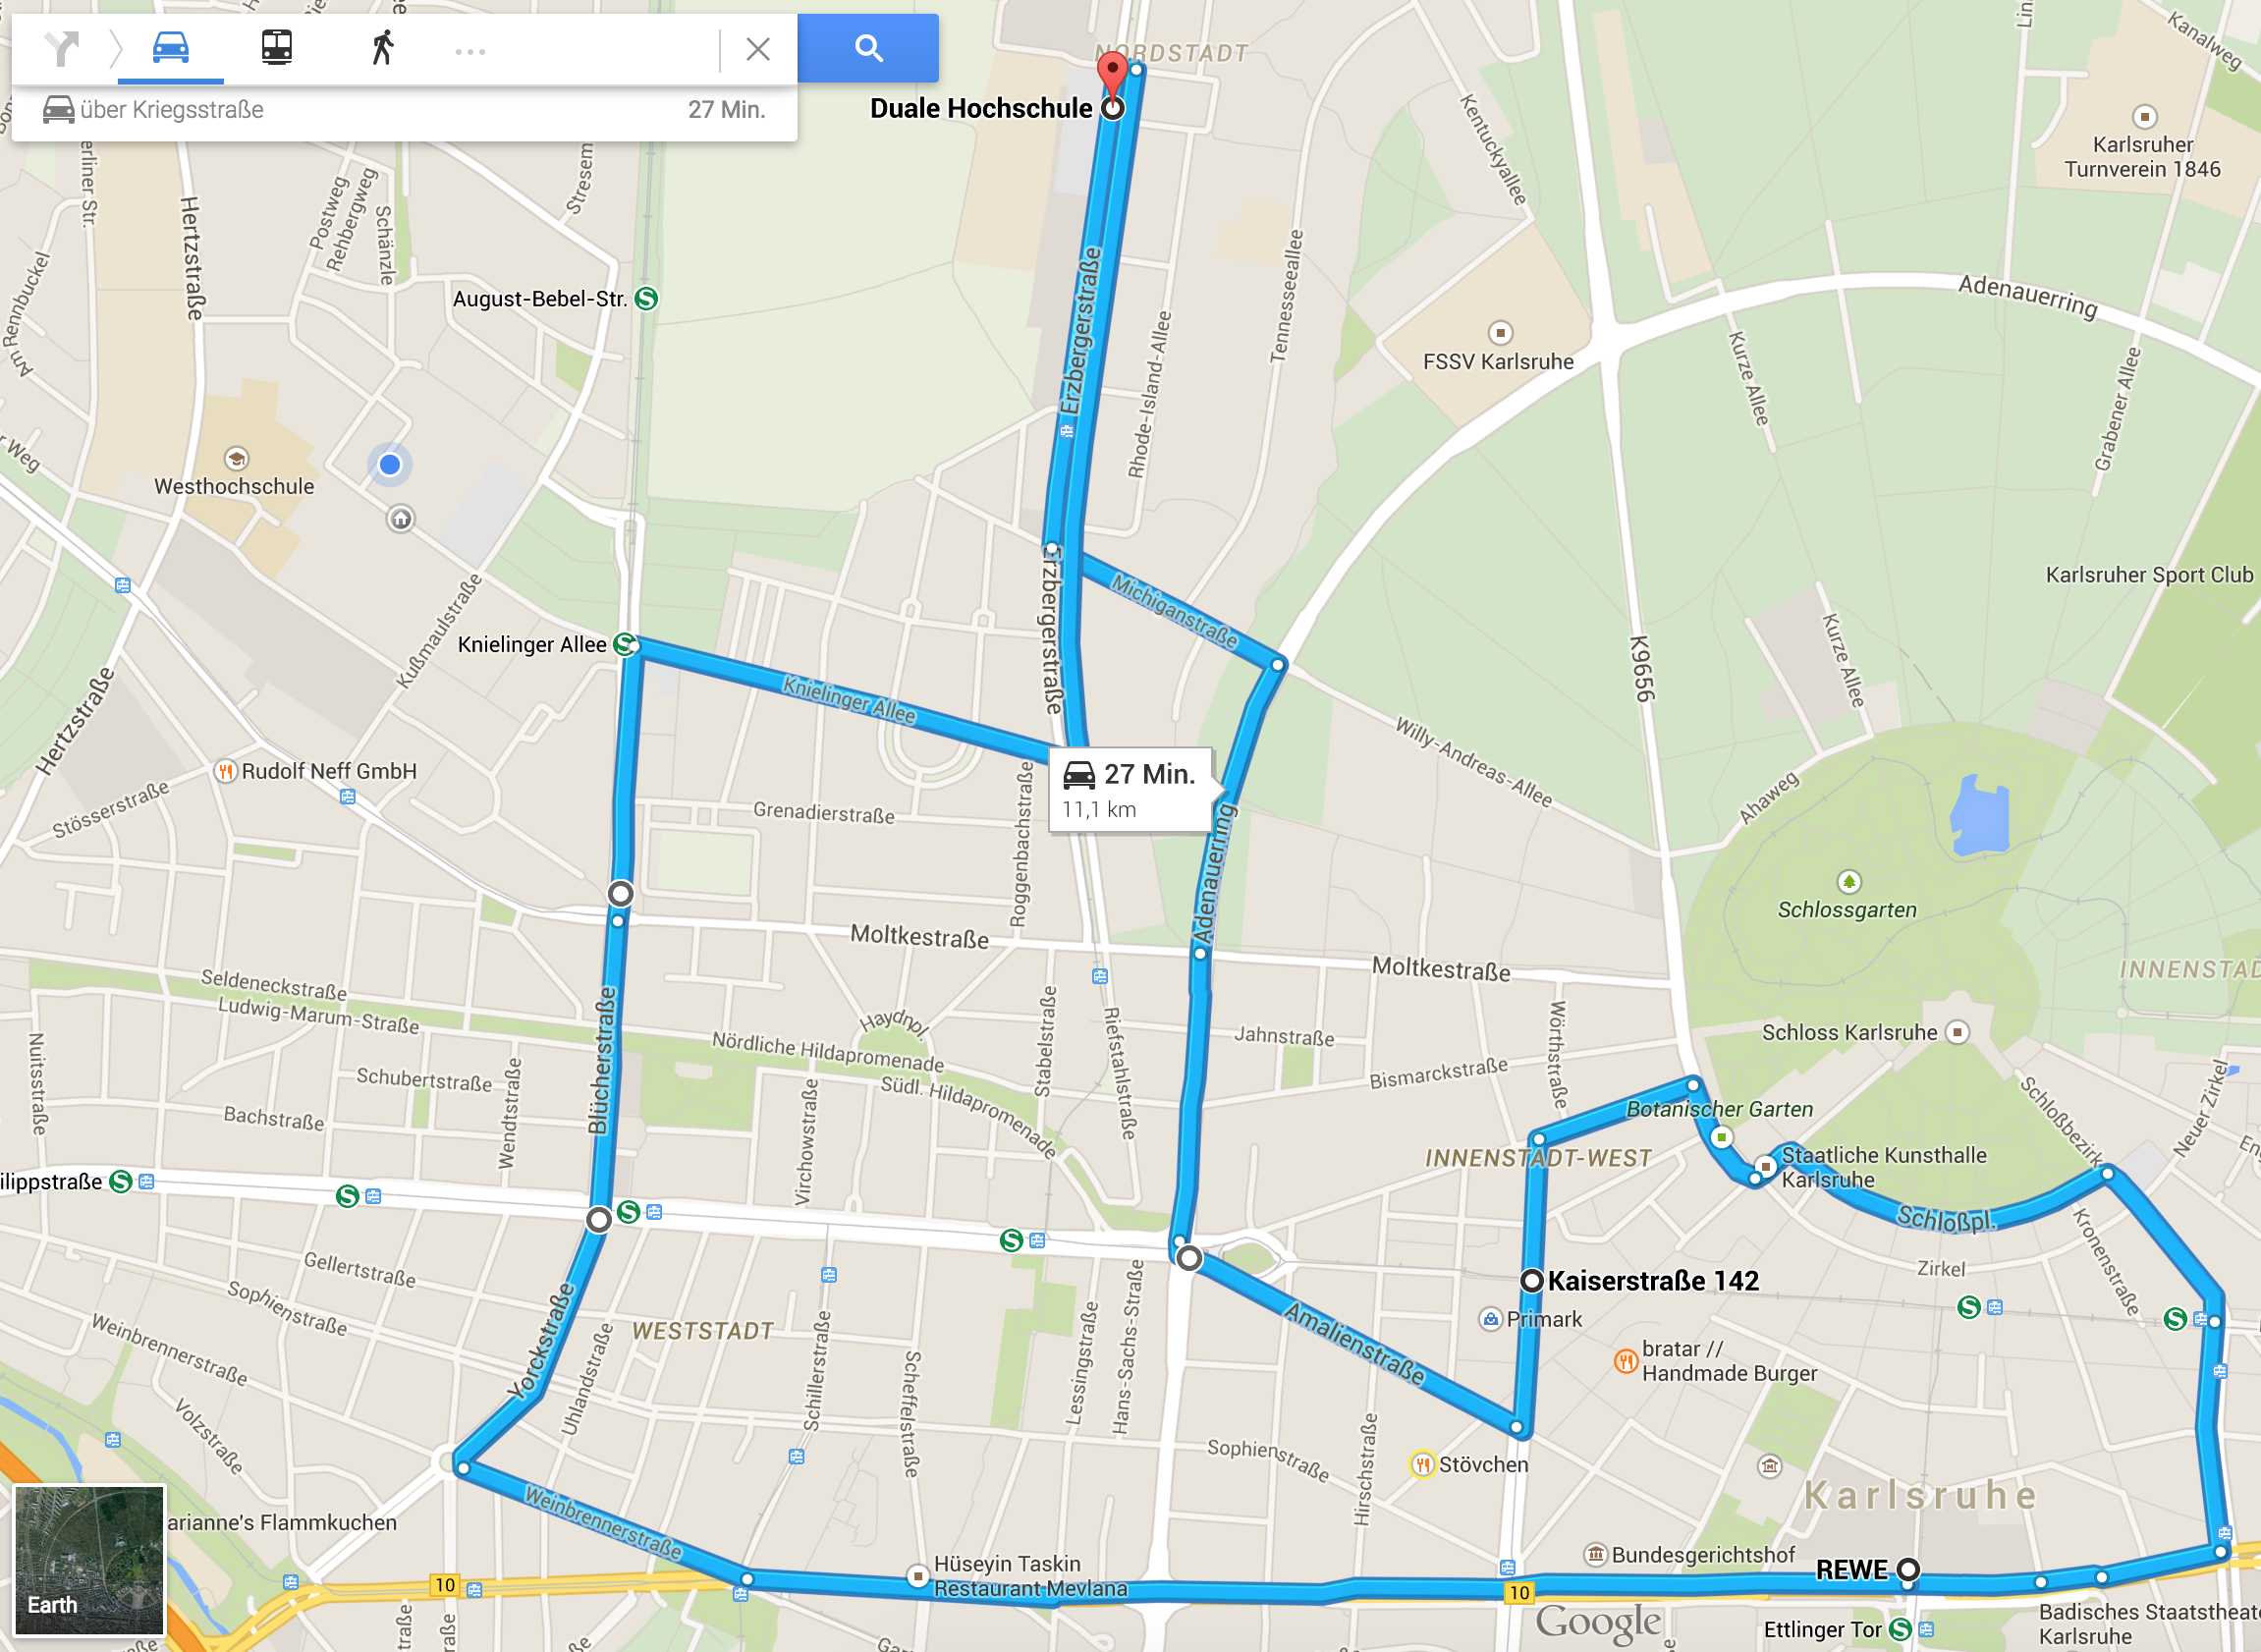
\includegraphics[width=\linewidth,height=150px,keepaspectratio]{alltag.png}
      \caption{Alltag für Viele}
    \end{figure}
  \end{frame}

  \begin{frame}
    \frametitle{Definition}
    Es gibt $N$ Städte.
    Zwischen zwei Städten $i$ und $j$ gibt es jeweils eine Kante $c_{ij}$.
    Sollte einmal keine Kante bestehen, so wird eine Kante mit großer Länge
    automatisch eingefügt.
  \end{frame}

  \begin{frame}
    \frametitle{TSP-Klassifikationen}
    \begin{itemize}[<+->]
      \item \textbf{Symmetrisches TSP}
        \linebreak
        Ungerichteter Graph
        $$c_{ij} = c_{ji}$$
        Hin- und Rückweg zwischen zwei Knotenpunkten stets gleich
      \item \textbf{Asymmetrisches TSP}
        \linebreak
        Gerichteter Graph
        Hin- und Rückweg zwischen zwei Knotenpunkten muss nicht gleich sein
      \item \textbf{Metrisches TSP}
        \linebreak
        Erfüllen der Dreiecksungleichung
        $$c_{ij} \le c_{ik} + c_{kj}$$
        Verbindung von $i$ nach $j$ nie länger als über dritten Knoten $k$
    \end{itemize}
  \end{frame}

  \begin{frame}
    \frametitle{Nicht-metrisches TSP}
    Ein TSP-Problem kann auch nicht-metrisch sein, wenn Umrüstzeiten
    berücksichtigt werden müssen.
    \pause
    Beispiel: Drei Trucks sollen an verschiedenen Stationen Gegenstände
    abliefern und aufnehmen:
    \begin{figure}
      \centering
      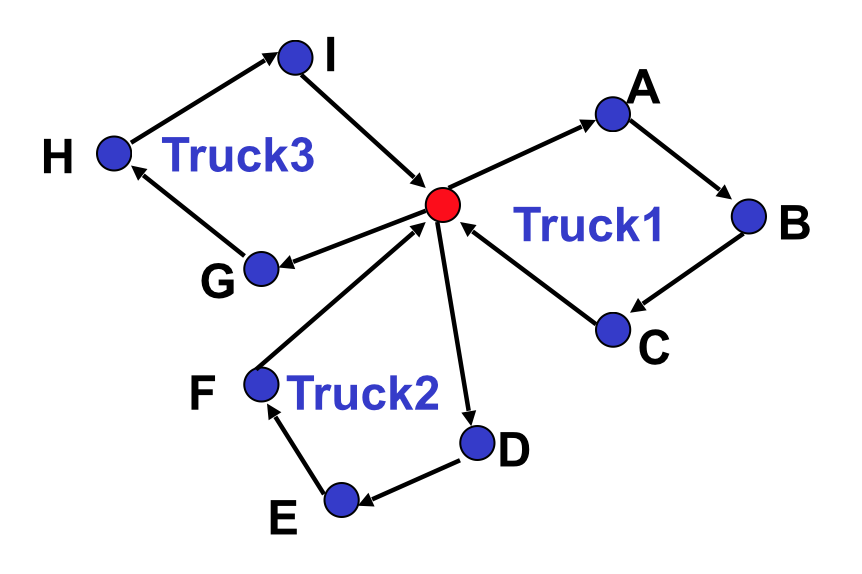
\includegraphics[width=\linewidth,height=150px,keepaspectratio]{truck_problem.png}
      \caption{Truck Problem}
    \end{figure}
  \end{frame}
% etc
\end{document}